\chapter{Cài đặt, thử nghiệm và đánh giá kết quả}
\label{ch:caidat}
\label{ch:ketqua}

Chương này trình bày phần hiện thực của hệ thống Uni Connect: môi trường triển khai,
các thành phần mã nguồn chính, giao diện người dùng thực tế, kết quả kiểm thử và kết
quả thực nghiệm của mô hình học máy. Nội dung chương là căn cứ để đối chiếu bốn mục
tiêu đã đặt ra ở Chương~\ref{ch:modau} với kết quả đo được.

\section{Môi trường triển khai}

Hệ thống được lập trình, huấn luyện và kiểm thử hoàn chỉnh trên môi trường máy chủ
cục bộ với các thông số cấu hình cụ thể:
\begin{itemize}[leftmargin=1.6em, itemsep=2pt]
  \item \textbf{Phần cứng:} Vi xử lý Intel Core i7 12 nhân 16 luồng, bộ nhớ trong RAM 16~GB DDR5, ổ cứng lưu trữ thể rắn NVMe SSD 512~GB.
  \item \textbf{Hệ điều hành:} Microsoft Windows 11 Home 64-bit kết hợp môi trường thực thi POSIX Git Bash.
  \item \textbf{Môi trường runtime:} Python 3.13.2 64-bit, quản lý gói thông qua \code{pip} và môi trường ảo \code{venv}.
  \item \textbf{Cơ sở dữ liệu:} MySQL Server 8.0 Community Edition, bảng mã lưu trữ \code{utf8mb4}.
  \item \textbf{Quản lý phiên bản:} Hệ thống kiểm soát phiên bản Git, lưu trữ kho mã nguồn tại GitHub (\url{https://github.com/tann299/DAU-2026-2027-Uni-Map}).
\end{itemize}

Bảng~\ref{tab:moitruong} đối chiếu cấu hình máy phát triển dùng để huấn luyện với cấu
hình máy chủ tối thiểu mà hệ thống cần để vận hành. Việc tách hai cấu hình này là có
chủ đích: huấn luyện mô hình đòi hỏi nhiều nhân CPU và RAM, trong khi phục vụ trực
tuyến chỉ cần nạp sẵn \code{model.pkl} vào bộ nhớ và trả kết quả cho từng truy vấn.

\begin{table}[H]
\centering
\caption{Đối chiếu cấu hình máy phát triển (huấn luyện) và máy chủ vận hành (phục vụ).}
\label{tab:moitruong}
\small
\begin{tabularx}{\textwidth}{@{}>{\raggedright\arraybackslash}p{3.1cm}
  >{\raggedright\arraybackslash}X
  >{\raggedright\arraybackslash}X@{}}
\toprule
\rowcolor{gray100}\bfseries\color{daunavy}Thành phần &
\bfseries\color{daumaroon}Máy phát triển (huấn luyện) &
\bfseries\color{daunavy}Máy chủ vận hành (tối thiểu) \\
\midrule
CPU        & Intel Core i7, 12 nhân / 16 luồng & 1 vCPU \\
RAM        & 16~GB DDR5                        & 2~GB \\
Lưu trữ    & NVMe SSD 512~GB                   & 20~GB (mã nguồn, CSDL, \code{model.pkl}) \\
Hệ điều hành & Windows 11 Home 64-bit          & Linux (Ubuntu 22.04 LTS) \\
Python     & 3.13.2                            & 3.13.x \\
MySQL      & 8.0 Community, \code{utf8mb4}     & 8.0, \code{utf8mb4} \\
Vai trò    & Chạy \code{crawl}, \code{gen\_dataset}, \code{train} & Chạy Django + Gunicorn, nạp mô hình vào RAM \\
\bottomrule
\end{tabularx}
\end{table}

Bảng~\ref{tab:moitruong} cho thấy toàn bộ yêu cầu tài nguyên của hệ thống nằm trong
ngưỡng một máy chủ VPS phổ thông: 1 vCPU và 2~GB RAM là đủ để phục vụ, vì chi phí
tính toán nặng (sinh đặc trưng, huấn luyện 100 cây) đã được đẩy ra khỏi vòng đời
truy vấn. Ràng buộc thực sự đáng kể là dung lượng RAM dành cho \code{model.pkl}
($\approx$~52~MB) và bộ đệm của MySQL; hai mục này chiếm phần lớn trong 2~GB nêu
trên. Cấu hình phát triển mạnh hơn chỉ cần thiết ở giai đoạn huấn luyện, khi
\code{train.py} chạy song song trên toàn bộ nhân CPU thông qua \code{n\_jobs = -1}.

Hình~\ref{fig:deploy} mô tả cách các thành phần trên được bố trí khi triển khai thật.

\begin{figure}[H]
\centering
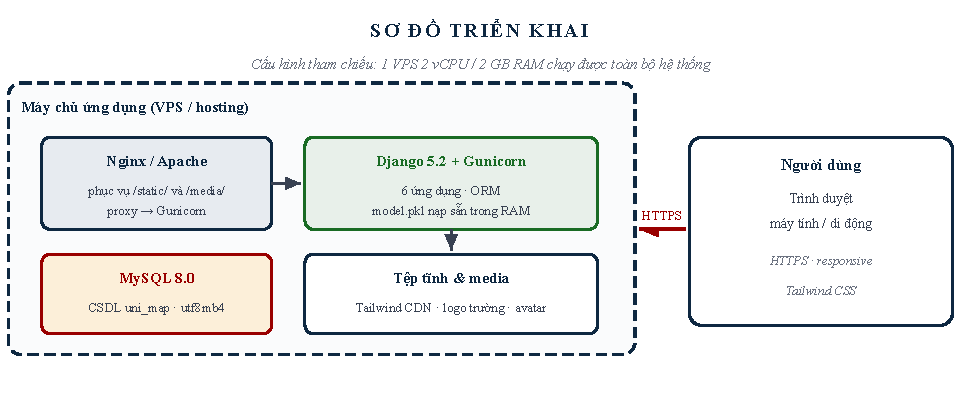
\includegraphics[width=\textwidth]{figs/svg/h-deploy.pdf}
\caption{Sơ đồ triển khai hệ thống trên một máy chủ VPS đơn lẻ.}
\label{fig:deploy}
\end{figure}

Trong Hình~\ref{fig:deploy}, máy chủ đứng sau một lớp Nginx/Apache đóng vai trò phục vụ
tệp tĩnh và chuyển tiếp yêu cầu động sang tiến trình Gunicorn chạy ứng dụng Django.
Tiến trình này nạp sẵn \code{model.pkl} vào RAM ngay khi khởi động, nên mỗi lượt gợi
ý chỉ còn chi phí vector hóa và gọi \code{predict\_proba}. MySQL 8.0 nằm cùng máy chủ
và chỉ được truy cập qua Django ORM; tệp tĩnh và media (logo trường, ảnh đại diện)
được phục vụ trực tiếp, không đi qua tầng ứng dụng. Toàn bộ đường truyền từ trình
duyệt tới máy chủ dùng HTTPS. Cách bố trí một máy chủ này phù hợp với quy mô đồ án,
đồng thời giữ nguyên khả năng tách tầng sau này: nếu lượng truy cập tăng, chỉ cần
chuyển MySQL sang máy riêng và nhân bản tiến trình Gunicorn mà không sửa mã nguồn.

\section{Các thành phần mã nguồn chính}

Kiến trúc mã nguồn được phân rã thành hai phân hệ độc lập: phân hệ xử lý dữ liệu
ngoại tuyến (\en{offline pipeline}) và phân hệ ứng dụng web trực tuyến
(\en{online service}). Hình~\ref{fig:pipeline} tóm tắt toàn bộ đường đi của dữ liệu
qua sáu bước của phân hệ ngoại tuyến.

\begin{figure}[H]
\centering
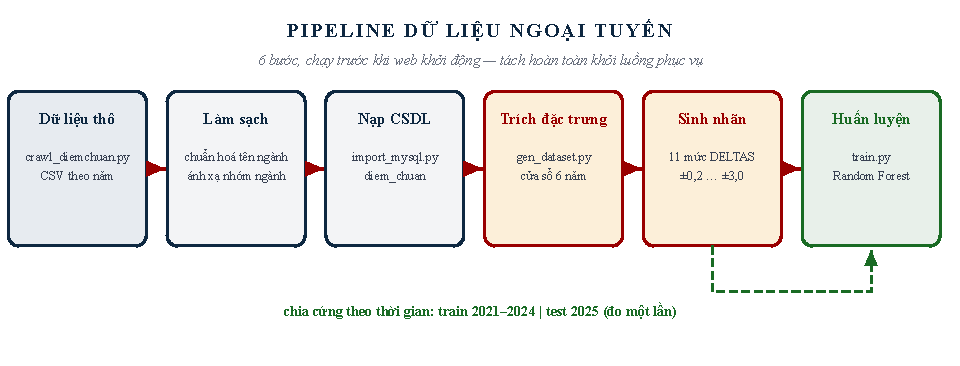
\includegraphics[width=\textwidth]{figs/svg/h-pipeline.pdf}
\caption{Pipeline dữ liệu ngoại tuyến gồm sáu bước, chạy trước khi web khởi động.}
\label{fig:pipeline}
\end{figure}

Sáu bước trong Hình~\ref{fig:pipeline} tương ứng sáu tệp mã nguồn độc lập, mỗi bước
ghi ra một đầu ra trung gian kiểm tra được. Bước 1 (\code{crawl\_diemchuan.py}) sinh
ra các tệp CSV theo năm; bước 2 làm sạch tên ngành và ánh xạ về 15 nhóm ngành chuẩn;
bước 3 nạp vào MySQL qua \code{import\_mysql.py}; bước 4 (\code{gen\_dataset.py})
trích đặc trưng từ cửa sổ sáu năm; bước 5 sinh nhãn bằng 11 mức \code{DELTAS}; bước 6
(\code{train.py}) huấn luyện và đóng gói mô hình. Điểm quan trọng là ranh giới thời
gian: dữ liệu được chia cứng thành tập huấn luyện 2021--2024 và tập kiểm thử 2025, và
phép chia này chỉ thực hiện đúng một lần để kết quả đo không bị nhiễu bởi việc chọn
lại tập kiểm thử.

\subsection{Pipeline tiền xử lý và sinh tập dữ liệu}

Module \code{gen\_dataset.py} thực hiện chuyển đổi chuỗi 10 năm điểm chuẩn từ bảng
quan hệ thành tập dữ liệu huấn luyện phẳng. Để ngăn chặn hoàn toàn rò rỉ dữ liệu, hàm
xử lý tính toán đặc trưng tại năm $t$ chỉ dựa trên cửa sổ lịch sử 6 năm trước đó
($t - \text{lookback} \le \text{năm} < t$) và áp dụng 11 mức chênh lệch điểm đối xứng
\code{DELTAS} để sinh mẫu thí sinh giả lập.

\begin{lstlisting}[language=Python, caption={Hàm sinh mẫu giả lập đối xứng và tách tập theo thời gian.}, label={lst:gendata}]
# Symmetric delta grid around true cutoff score (constants.py)
DELTAS = [-3.0, -2.0, -1.0, -0.5, -0.2, 0.0, 0.2, 0.5, 1.0, 2.0, 3.0]
NAM_LOOKBACK = 6

def build_split(df_history, target_year):
    """Generate training rows for target_year using only years < target_year."""
    valid_window = [y for y in range(target_year - NAM_LOOKBACK, target_year)]
    features = extract_window_features(df_history, valid_window)

    # Expand each application row across 11 synthetic candidates
    expanded_rows = []
    for _, row in features.iterrows():
        cutoff = row["diem_chuan_target"]
        for d in DELTAS:
            sim_score = cutoff + d
            label = 1 if sim_score >= cutoff else 0
            expanded_rows.append({
                **row.to_dict(),
                "diem_thi": sim_score,
                "margin": d,
                "nhan": label
            })
    return pd.DataFrame(expanded_rows)
\end{lstlisting}

Mã nguồn~\ref{lst:gendata} cho thấy hai quyết định kỹ thuật được thể hiện trực tiếp
trong vòng lặp. Thứ nhất, \code{valid\_window} bị chặn trên bởi \code{target\_year}
nên không một giá trị nào của năm mục tiêu lọt vào vector đặc trưng. Thứ hai, nhãn
được suy ra từ chính \code{cutoff} của năm mục tiêu chứ không từ dữ liệu quá khứ, nên
nhãn và đặc trưng nằm ở hai mốc thời gian khác nhau đúng như thiết kế. Mỗi dòng lịch
sử được nhân thành 11 dòng huấn luyện, nhờ đó tỉ lệ hai lớp gần cân bằng mà không cần
kỹ thuật lấy mẫu bù.

\subsection{Huấn luyện mô hình và tối ưu kích thước lưu trữ}

Quy trình huấn luyện trong \code{train.py} thực hiện chuẩn hóa dữ liệu bằng
\code{StandardScaler} và huấn luyện mô hình \code{RandomForestClassifier}. Để đáp ứng
ràng buộc lưu trữ dưới 100~MB (nhằm đưa vào bộ nhớ RAM máy chủ phổ thông), số lượng
cây được chốt ở 100 và độ sâu tối đa được giới hạn ở mức 14.

\begin{lstlisting}[language=Python, caption={Quy trình huấn luyện và đóng gói mô hình.}, label={lst:train}]
from sklearn.ensemble import RandomForestClassifier
from sklearn.preprocessing import StandardScaler
import joblib

def train_and_export(X_train, y_train, export_dir="ml/"):
    """Fit scaler and Random Forest model, then export serialized weights."""
    scaler = StandardScaler().fit(X_train)
    Z_train = scaler.transform(X_train)

    # 100 estimators, max depth 14 limits pkl file size to ~52 MB
    rf = RandomForestClassifier(
        n_estimators=100,
        min_samples_leaf=5,
        max_depth=14,
        n_jobs=-1,
        random_state=42
    )
    rf.fit(Z_train, y_train)

    joblib.dump(rf, f"{export_dir}/model.pkl", compress=3)
    joblib.dump(scaler, f"{export_dir}/scaler.pkl")
    return rf, scaler
\end{lstlisting}

Điểm đáng chú ý trong Mã nguồn~\ref{lst:train} là bộ chuẩn hóa \code{scaler} được lưu
thành một tệp riêng thay vì gộp vào mô hình. Khi suy luận, ứng dụng web phải nạp lại
đúng bộ chuẩn hóa này để biến đổi vector đầu vào theo cùng tham số trung bình và độ
lệch chuẩn đã dùng lúc huấn luyện; nếu thiếu bước đó, \code{StandardScaler} sẽ dùng
tham số mặc định và toàn bộ dự đoán sai lệch. Tham số \code{compress=3} của
\code{joblib} giảm kích thước tệp còn khoảng 52~MB mà thời gian nạp vẫn dưới một giây,
phù hợp với yêu cầu nạp một lần lúc khởi động.

\subsection{Động cơ suy luận và cơ chế chịu lỗi}

Tại tầng ứng dụng web Django, tệp \code{predict.py} nạp mô hình vào bộ nhớ RAM dưới
dạng biến toàn cục để tránh chi phí I/O đọc đĩa cứng trong mỗi lượt truy vấn của
người dùng. Khi nhận danh sách các ngành ứng viên, mô hình thực hiện dự đoán theo lô
(\en{batch prediction}) bằng phương thức \code{predict\_proba}, đảm bảo thời gian xử
lý toàn bộ 30 nguyện vọng dưới 50 mili-giây.

\begin{lstlisting}[language=Python, caption={Hàm chấm xác suất theo lô và cơ chế dự phòng.}, label={lst:predict}]
_CACHE = {"model": None, "scaler": None}

def cham_xac_suat(ds_nguyen_vong, diem_thi):
    """Batch inference with graceful fallback to margin ranking."""
    try:
        if _CACHE["model"] is None:
            _CACHE["model"] = joblib.load("ml/model.pkl")
            _CACHE["scaler"] = joblib.load("ml/scaler.pkl")

        # Build 27-dim feature matrix Z for all candidates at once
        X = vector_hoa_hang_loat(ds_nguyen_vong, diem_thi)
        Z = _CACHE["scaler"].transform(X)
        probs = _CACHE["model"].predict_proba(Z)[:, 1]
        return probs, "AI_RANDOM_FOREST"
    except Exception as e:
        # Fallback to deterministic margin sorting when model fails
        margins = [diem_thi - nv["diem_moi_nhat"] for nv in ds_nguyen_vong]
        return margins, "FALLBACK_MARGIN"
\end{lstlisting}

Mã nguồn~\ref{lst:predict} là hiện thực của yêu cầu phi chức năng về độ tin cậy: khối
\code{try} bao trọn cả bước nạp mô hình, vector hóa và suy luận, nên mọi sự cố (thiếu
tệp, sai phiên bản thư viện, lỗi định dạng) đều rơi vào cùng một nhánh xử lý. Nhánh
\code{except} không trả về lỗi mà chuyển sang xếp hạng theo \code{margin} thuần và
đánh dấu nguồn kết quả là \code{FALLBACK\_MARGIN}; nhãn này được truyền xuống giao
diện để người dùng biết kết quả hiện tại không đến từ mô hình AI. Nhờ vậy hệ thống
luôn trả về mã HTTP 200 kèm một danh sách gợi ý hợp lệ, đúng với cam kết ở
Mục~\ref{sec:nfr}.

\section{Giao diện và kịch bản sử dụng}

Ứng dụng web được xây dựng với phong cách trực quan, tối ưu cho cả máy tính để bàn và
thiết bị di động bằng framework Tailwind CSS. Cấu trúc trang được bố trí gồm 4 phân
khu chính:

\begin{enumerate}[leftmargin=1.6em, itemsep=2pt]
  \item \textbf{Trang tra cứu thông tin trường và ngành:} Cho phép lọc nhanh 295 trường theo 3 vùng miền, loại hình công lập/tư thục và xem chuỗi 10 năm điểm chuẩn trực quan (Hình~\ref{fig:demo-tracuu}).
  \item \textbf{Trang quản lý hồ sơ điểm cá nhân:} Thí sinh nhập điểm các môn thi THPT hoặc điểm học bạ lớp 12. Hệ thống tự động tính toán tổng điểm cho tất cả các tổ hợp xét tuyển hợp lệ (Hình~\ref{fig:demo-hoso}).
  \item \textbf{Trang gợi ý nguyện vọng AI:} Hiển thị danh sách nguyện vọng được sắp xếp theo xác suất giảm dần và phân thành 3 khối màu rõ rệt: Tầng \textbf{An toàn} (màu xanh lá, $p \ge 0{,}80$), Tầng \textbf{Vừa sức} (màu xanh dương, $0{,}40 \le p < 0{,}80$) và Tầng \textbf{Thử sức} (màu cam, $p < 0{,}40$). Mỗi hàng đi kèm thẻ giải thích nguyên nhân ngắn gọn. Giao diện thực tế của trang này thể hiện ở Hình~\ref{fig:demo-goiy}.
  \item \textbf{Trang quản trị hệ thống:} Dành cho quản trị viên theo dõi số lượng bản ghi dữ liệu, kích hoạt pipeline chạy ngầm cập nhật dữ liệu và thực hiện huấn luyện lại mô hình trực tiếp trên giao diện (Hình~\ref{fig:demo-admin}).
\end{enumerate}

\begin{figure}[H]
\centering
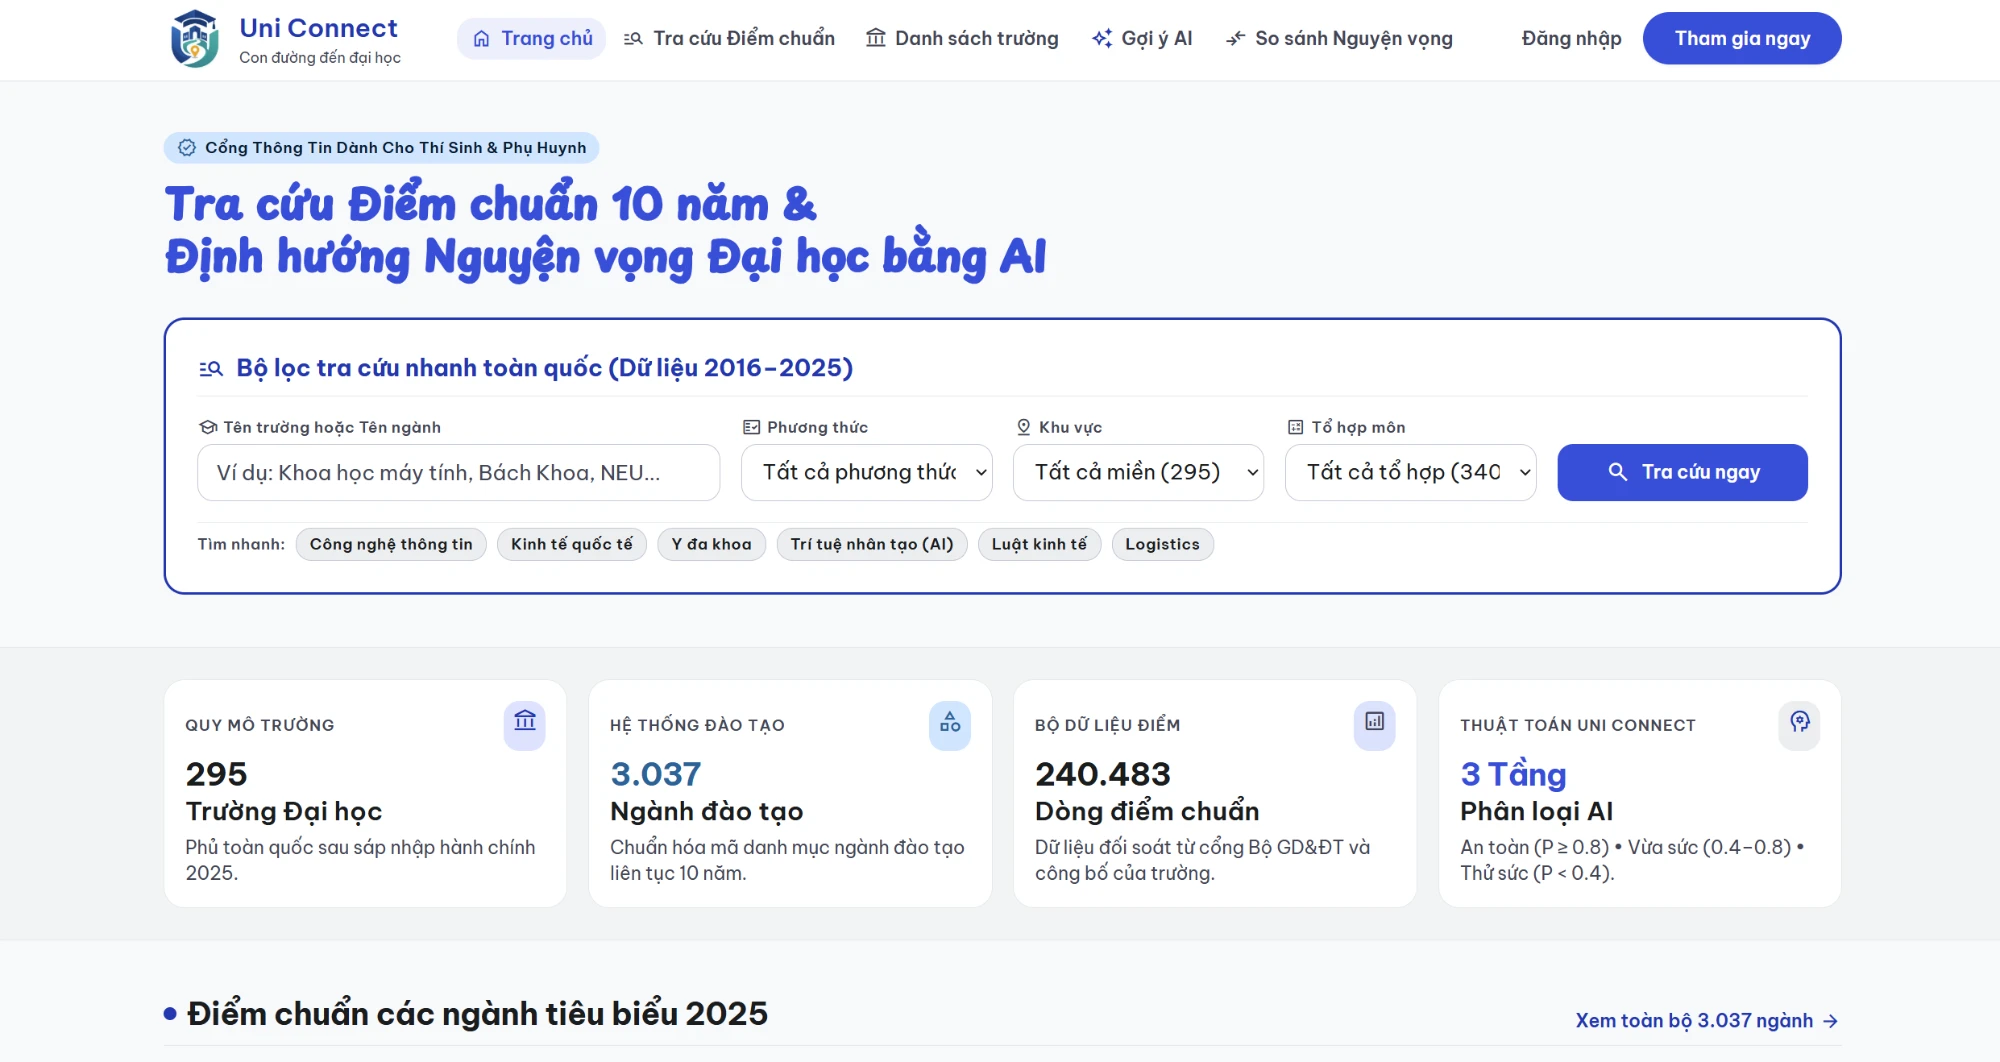
\includegraphics[width=\textwidth]{figs/uniconnect-p1.png}
\caption{Giao diện trang chủ Uni Connect --- tra cứu điểm chuẩn 10 năm.}
\label{fig:demo-tracuu}
\end{figure}

Hình~\ref{fig:demo-tracuu} là trang chủ của hệ thống. Phần đầu trang đặt ô tìm kiếm
theo tên trường, ngành hoặc mã trường kèm bốn bộ lọc (tỉnh thành, tổ hợp môn, nhóm
ngành, phương thức). Bên dưới là bốn ô thống kê lấy trực tiếp từ cơ sở dữ liệu: 295
trường, 3.037 ngành, 240.483 dòng điểm và 3 tầng gợi ý. Bảng điểm chuẩn ở cuối trang
hiển thị song song ba năm gần nhất cùng cột biến động, cho phép người dùng nhận ra xu
hướng tăng giảm ngay ở màn hình đầu tiên mà không phải mở trang chi tiết.

\begin{figure}[H]
\centering
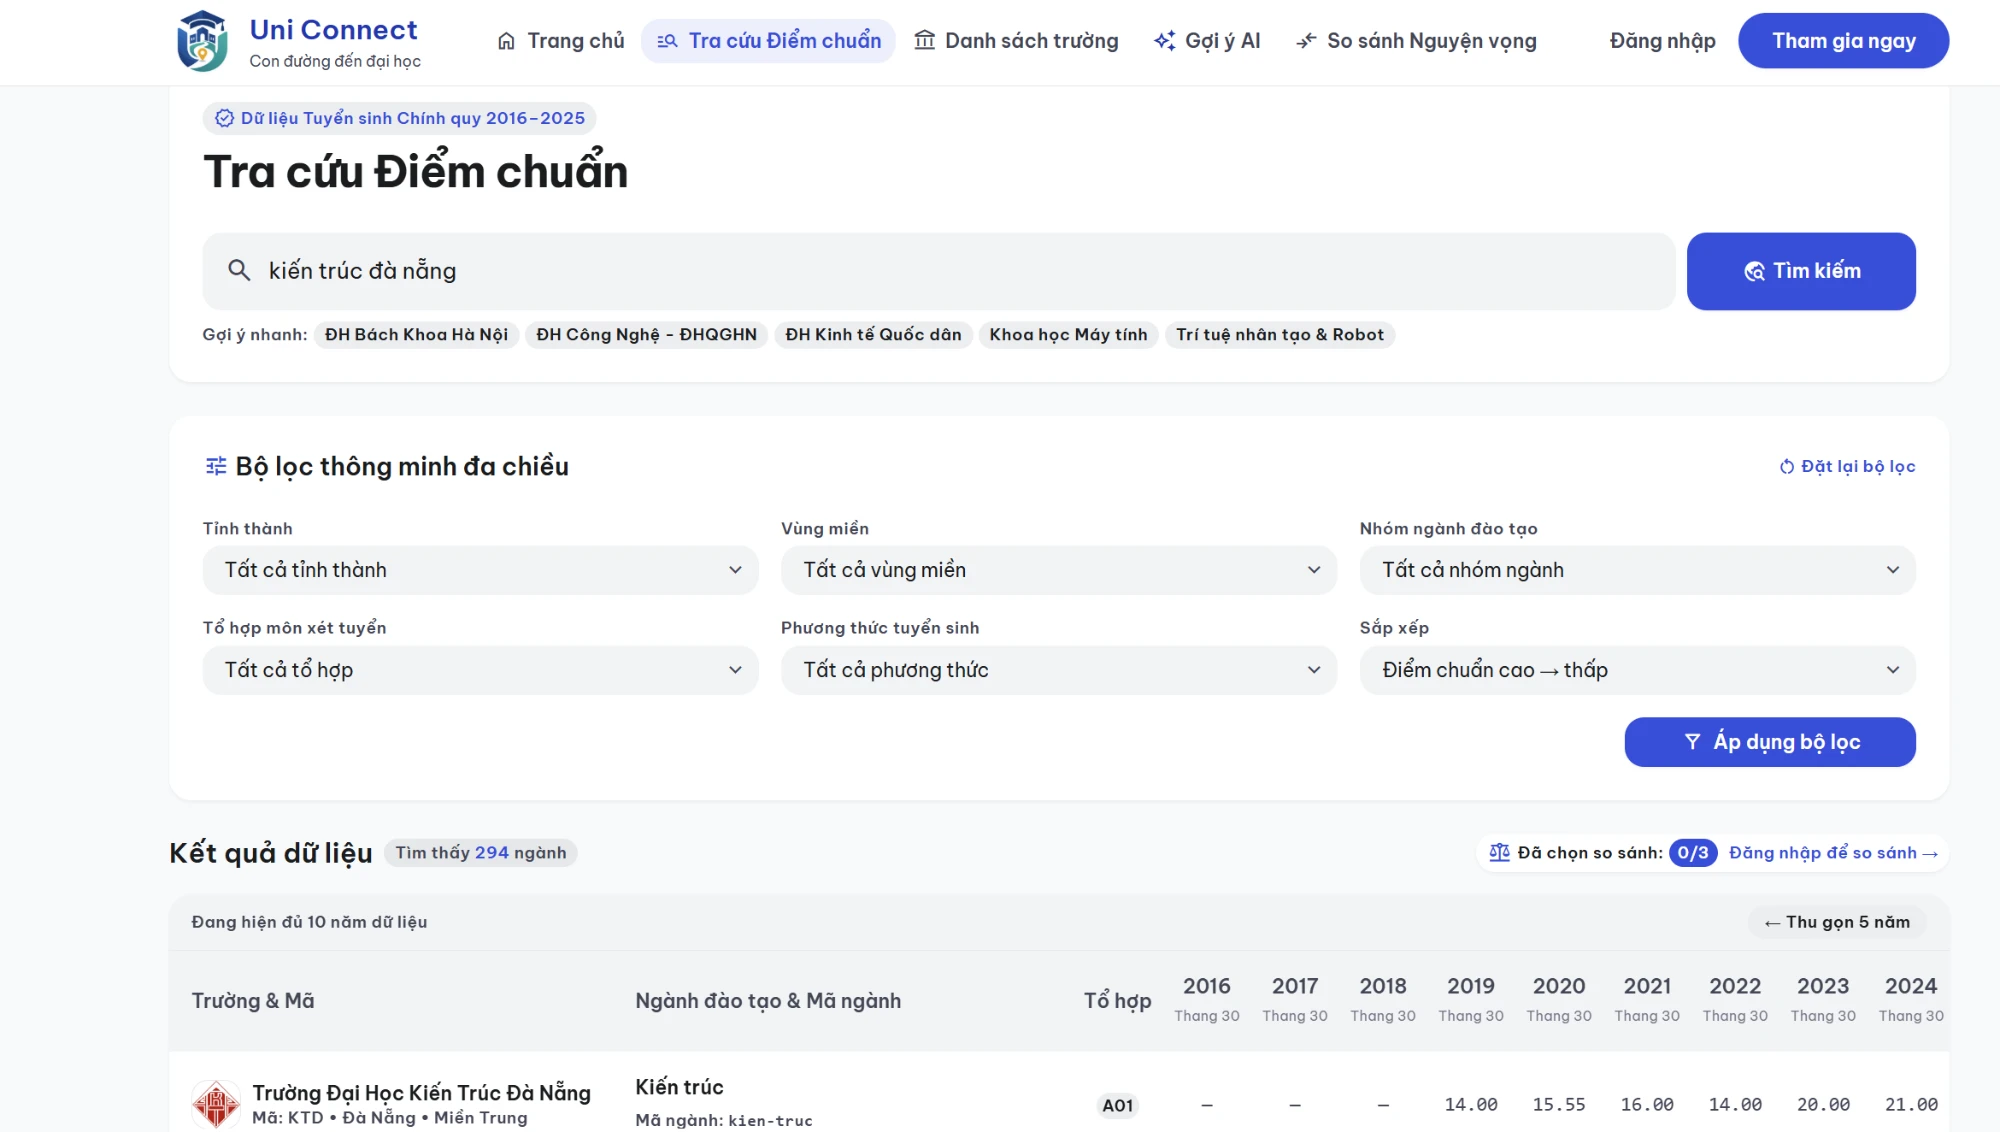
\includegraphics[width=\textwidth]{figs/uniconnect-p2.png}
\caption{Giao diện trang tra cứu điểm chuẩn đa tiêu chí.}
\label{fig:demo-hoso}
\end{figure}

Hình~\ref{fig:demo-hoso} là trang tra cứu chi tiết. Mỗi dòng kết quả gồm tên trường,
mã trường, tên ngành, tổ hợp xét tuyển và chuỗi điểm của các năm. Cột ngoài cùng bên
phải gắn nhãn xu hướng (tăng, giảm, ổn định) được tính từ hồi quy tuyến tính trên
chuỗi điểm, giúp thí sinh so sánh nhanh mức độ cạnh tranh giữa các ngành thay vì chỉ
nhìn một con số của năm gần nhất.

\begin{figure}[H]
\centering
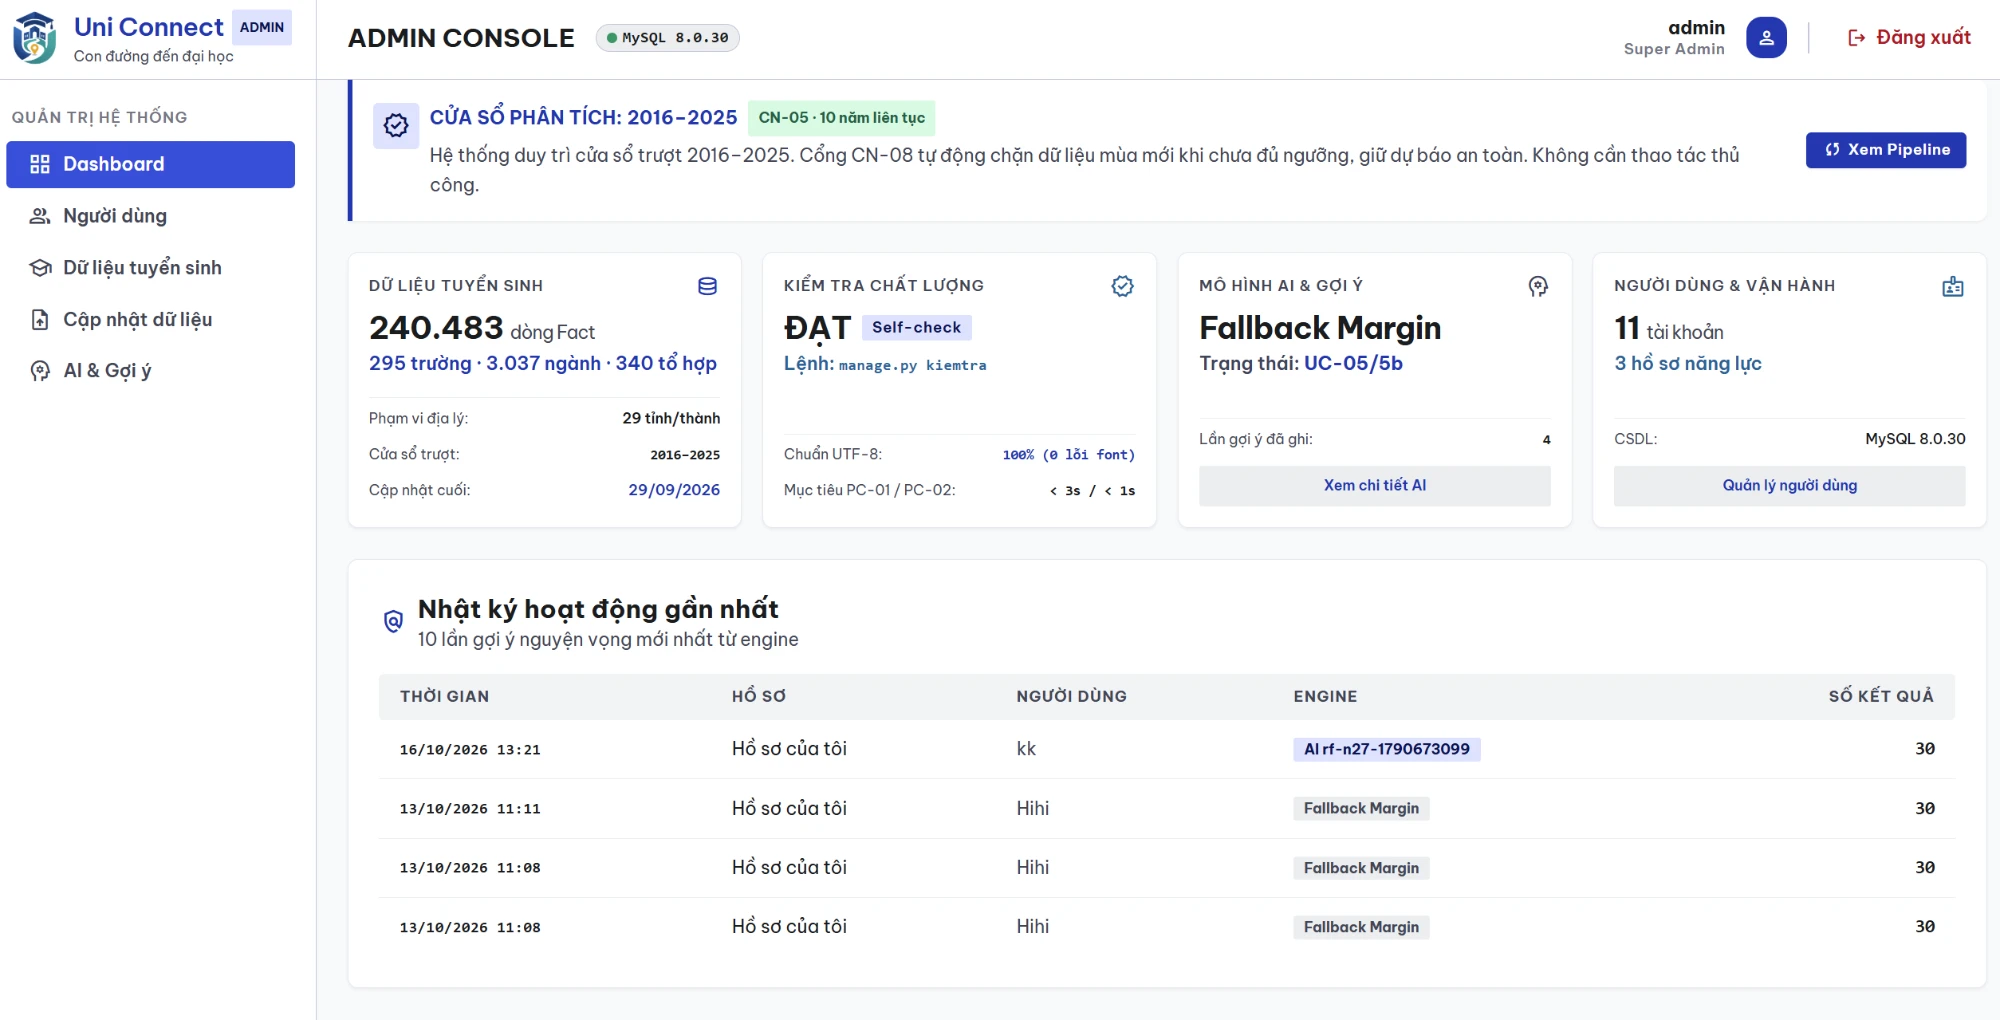
\includegraphics[width=\textwidth]{figs/uniconnect-p4.png}
\caption{Giao diện bảng điều khiển quản trị hệ thống (Admin Console).}
\label{fig:demo-admin}
\end{figure}

Hình~\ref{fig:demo-admin} là bảng điều khiển dành cho quản trị viên. Bốn thẻ đầu trang
tổng hợp trạng thái hệ thống: số dòng dữ liệu, kết quả tự kiểm tra chất lượng, trạng
thái mô hình AI và thông tin người dùng. Bảng nhật ký phía dưới ghi lại từng lần chạy
gợi ý kèm nguồn xử lý (\code{AI\_RANDOM\_FOREST} hoặc \code{FALLBACK\_MARGIN}), nhờ
đó có thể phát hiện ngay nếu mô hình gặp sự cố trong vận hành thực tế.

\begin{figure}[H]
\centering
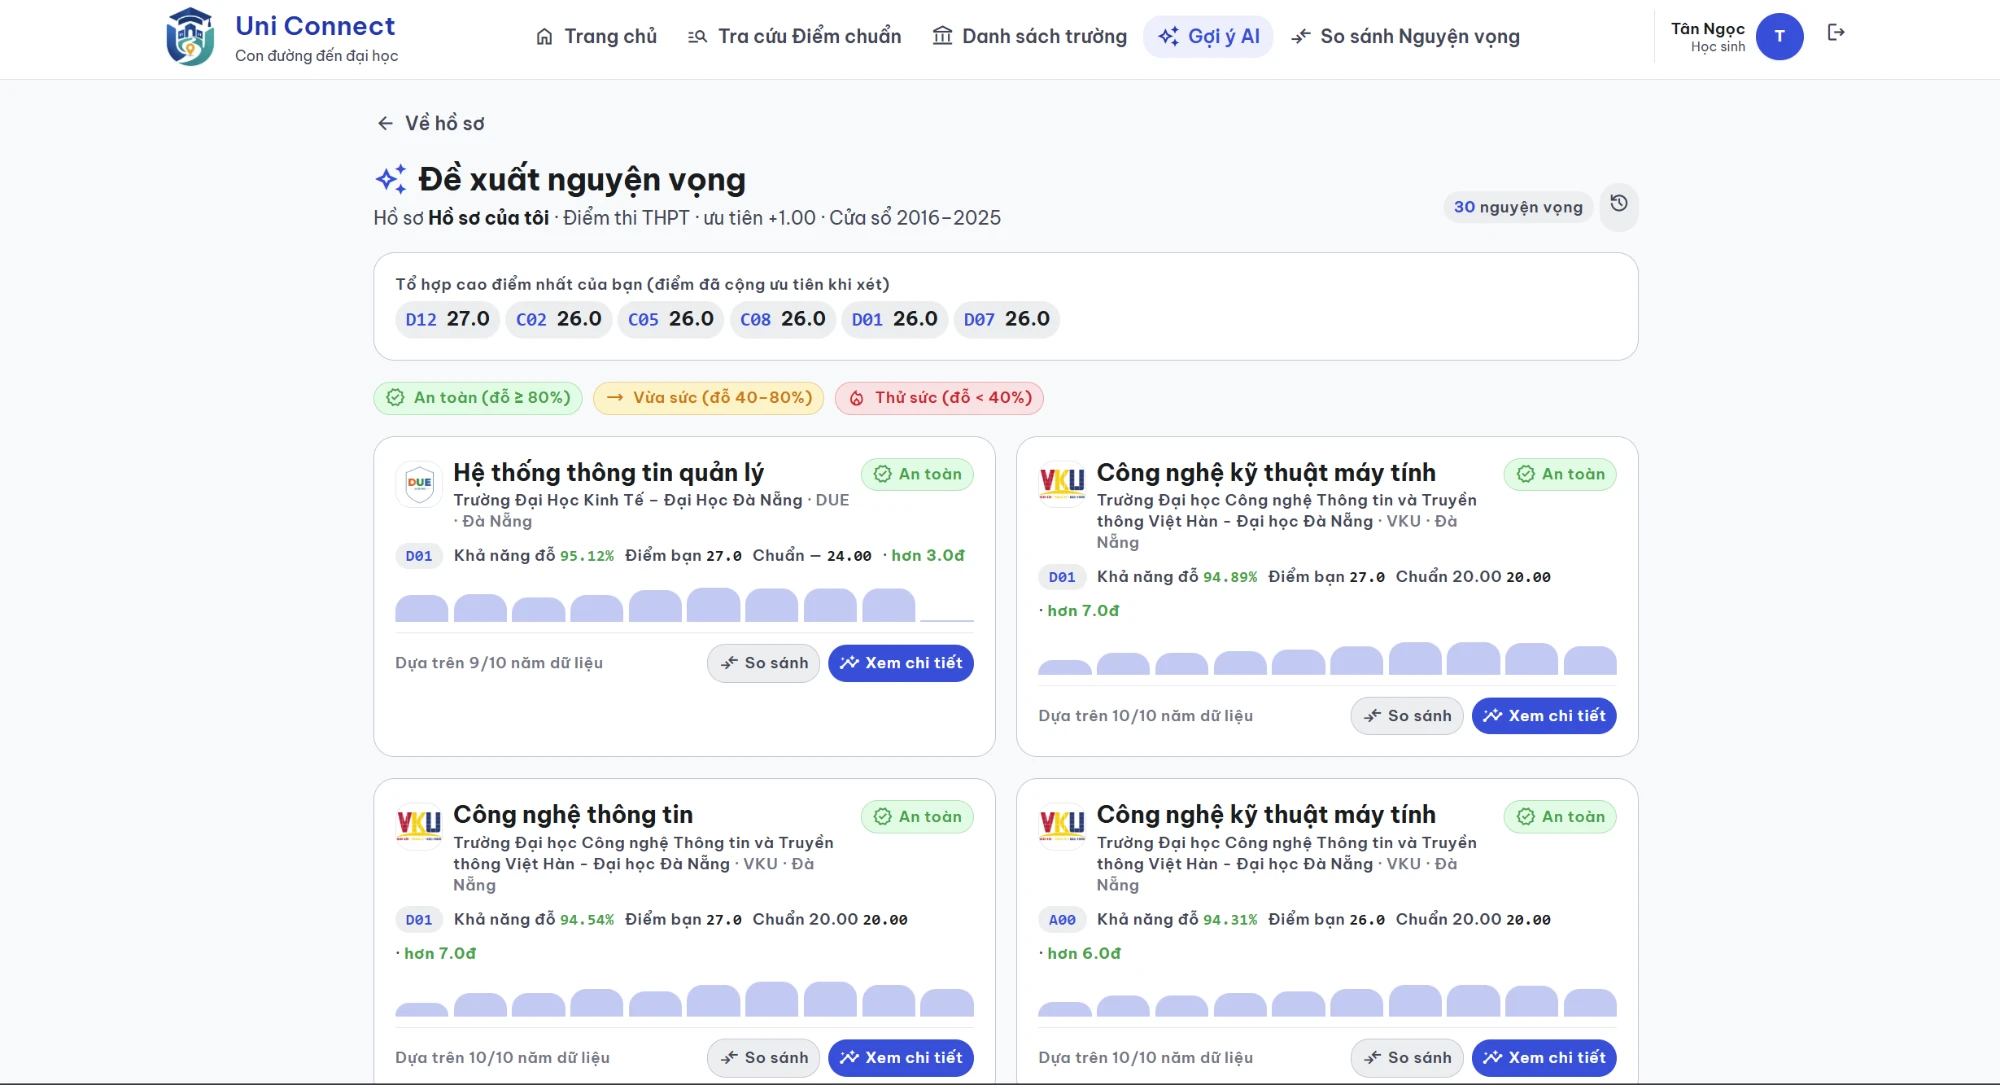
\includegraphics[width=\textwidth]{figs/uniconnect-goiy.png}
\caption{Giao diện trang gợi ý nguyện vọng AI với phân tầng An toàn, Vừa sức, Thử sức.}
\label{fig:demo-goiy}
\end{figure}

Hình~\ref{fig:demo-goiy} là màn hình trung tâm của hệ thống. Ba tab ở đầu trang tương
ứng ba tầng và ghi rõ ngưỡng xác suất ngay trên nhãn, nên người dùng không phải tự
đoán ý nghĩa màu sắc. Mỗi thẻ nguyện vọng hiển thị tên ngành, trường, tổ hợp, khả
năng đỗ, điểm của bản thân so với điểm chuẩn mới nhất, giá trị \code{margin} và đồ thị
chuỗi 10 năm. Những con số này chính là đầu vào của mô hình, được hiển thị lại để lời
gợi ý có thể kiểm chứng được thay vì là một kết quả hộp đen.

\section{Kiểm thử hệ thống}

Chất lượng và độ ổn định của hệ thống được kiểm chứng qua ba cấp độ kiểm thử: kiểm
thử đơn vị (\en{unit test}), kiểm thử tích hợp (\en{integration test}) và kiểm thử
khả năng chịu lỗi (\en{fault tolerance}). Hình~\ref{fig:testing} mô tả phạm vi của
từng cấp độ.

\begin{figure}[H]
\centering
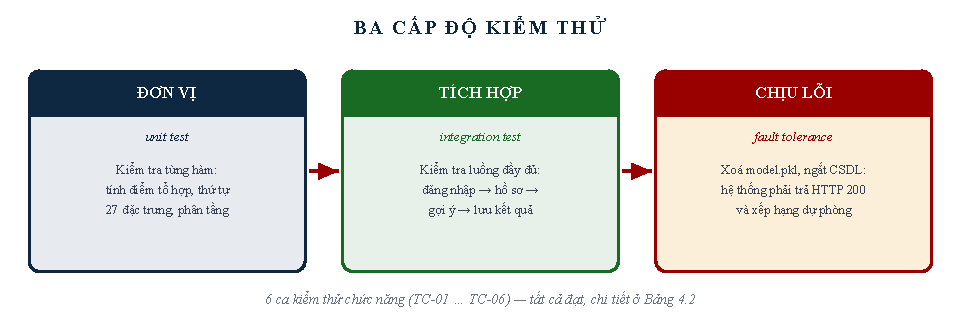
\includegraphics[width=\textwidth]{figs/svg/h-testing.pdf}
\caption{Ba cấp độ kiểm thử áp dụng cho hệ thống Uni Connect.}
\label{fig:testing}
\end{figure}

Ba cấp độ trong Hình~\ref{fig:testing} được thiết kế để phủ những rủi ro khác nhau.
Kiểm thử đơn vị kiểm tra từng hàm thuần túy --- tính tổng điểm tổ hợp, thứ tự 27 đặc
trưng, quy tắc gán tầng --- nơi lỗi thường là lỗi công thức và dễ tái hiện. Kiểm thử
tích hợp đi theo một luồng đầy đủ từ đăng nhập, nhập hồ sơ, gọi gợi ý đến lưu kết quả,
nhằm bắt lỗi ở các điểm nối giữa các tầng. Kiểm thử chịu lỗi cố tình phá vỡ điều kiện
bình thường (xóa \code{model.pkl}, ngắt kết nối CSDL) để xác nhận hệ thống vẫn trả về
mã HTTP 200 cùng kết quả dự phòng thay vì sập.

\begin{table}[H]
\centering
\caption{Kịch bản và kết quả các ca kiểm thử chính của hệ thống Uni Connect.}
\label{tab:kiemthu}
\small
\begin{tabularx}{\textwidth}{@{}>{\bfseries\color{daunavy}\raggedright\arraybackslash}m{2.45cm}
  >{\raggedright\arraybackslash}X
  >{\raggedright\arraybackslash}X
  >{\centering\arraybackslash}m{1.75cm}@{}}
\toprule
\rowcolor{gray100}\bfseries\color{daunavy}Mã kiểm thử & \bfseries\color{daunavy}Mục đích kiểm tra & \bfseries\color{daunavy}Kết quả kỳ vọng & \bfseries\color{daumaroon}Trạng thái \\
\midrule
TC-01 & Kiểm tra tính toán tổng điểm tổ hợp & Điểm cộng chính xác từng môn, đúng công thức hệ số & Đạt \\
TC-02 & Kiểm tra tính nhất quán 27 đặc trưng & Thứ tự cột vector khớp tuyệt đối với file \code{constants.py} & Đạt \\
TC-03 & Kiểm tra suy luận hàng loạt & Đầu ra đủ xác suất cho $N$ nguyện vọng, $0 \le p \le 1$ & Đạt \\
TC-04 & Kiểm tra phân tầng xác suất & Gán đúng 3 nhãn An toàn, Vừa sức, Thử sức theo ngưỡng & Đạt \\
TC-05 & Thử nghiệm khi thiếu file \code{model.pkl} & Chuyển sang xếp hạng \code{margin}, mã HTTP 200, không bị lỗi 500 & Đạt \\
TC-06 & Kiểm tra thời gian đáp ứng (PC-01) & Thời gian trả lời toàn bộ trang gợi ý dưới 3 giây; đo thực tế 0,42 giây & Đạt \\
\bottomrule
\end{tabularx}
\end{table}

Bảng~\ref{tab:kiemthu} tổng hợp kết quả của sáu ca kiểm thử chức năng, mỗi ca tương
ứng một rủi ro cụ thể. TC-01 và TC-02 bảo vệ tính đúng đắn của dữ liệu đầu vào mô
hình: một sai lệch thứ tự cột sẽ khiến mô hình nhận nhầm đặc trưng và cho ra xác suất
vô nghĩa dù không hề báo lỗi. TC-03 và TC-04 kiểm tra đầu ra, bảo đảm mọi giá trị xác
suất nằm trong $[0, 1]$ và nhãn tầng được gán đúng theo ngưỡng công bố. TC-05 là ca
quan trọng nhất về mặt vận hành: khi cố tình xóa tệp nhị phân của mô hình, hệ thống
không làm gián đoạn trải nghiệm người dùng mà ngay lập tức trả về danh sách sắp xếp
theo khoảng cách điểm kèm thông báo giải thích rõ ràng. TC-06 xác nhận chỉ tiêu hiệu
năng PC-01 với thời gian đo thực tế 0,42 giây, thấp hơn ngưỡng 3 giây gần bảy lần.

\section{Kết quả đạt được}

Bảng~\ref{tab:muctieu} đối chiếu trực tiếp bốn mục tiêu nêu tại
Chương~\ref{ch:modau} với kết quả đo được và ngưỡng đã cam kết.

\begin{table}[H]
\centering
\caption{Đối chiếu mục tiêu đặt ra với kết quả thực tế của đồ án.}
\label{tab:muctieu}
\small
\begin{tabularx}{\textwidth}{@{}>{\raggedright\arraybackslash}p{2.6cm}
  >{\raggedright\arraybackslash}p{3.5cm}
  >{\raggedright\arraybackslash}X
  >{\centering\arraybackslash}p{1.9cm}@{}}
\toprule
\rowcolor{gray100}\bfseries\color{daunavy}Mục tiêu &
\bfseries\color{daunavy}Ngưỡng đề ra &
\bfseries\color{daumaroon}Kết quả đo được &
\bfseries\color{daunavy}Đánh giá \\
\midrule
1. Dữ liệu & $\ge$ 250 trường; $\ge$ 3.000 ngành; $\ge$ 200.000 bản ghi &
295 trường; 3.037 ngành; 240.483 bản ghi điểm chuẩn 10 năm (2016--2025) &
Vượt mức \\
\addlinespace[2pt]
2. Mô hình AI & Accuracy $>$ 70\%; ROC-AUC $>$ 0,80 &
Accuracy 74,56\%; ROC-AUC 0,8354 trên tập kiểm thử độc lập 2025 &
Đạt \\
\addlinespace[2pt]
3. Phân tầng và giải thích & 3 tầng theo $p$; mỗi gợi ý có lời giải thích &
Ba tầng 0,80 / 0,40 vận hành ổn định; lời giải thích sinh từ \code{margin}, \code{xu_huong}, \code{bien_dong} &
Đạt \\
\addlinespace[2pt]
4. Ứng dụng web & Django $+$ MySQL; phản hồi $<$ 3 giây &
Đủ bốn phân khu chức năng; thời gian phản hồi đo được 0,42 giây &
Đạt \\
\bottomrule
\end{tabularx}
\end{table}

Bảng~\ref{tab:muctieu} cho thấy cả bốn mục tiêu đều đạt hoặc vượt ngưỡng. Mục tiêu dữ
liệu vượt ở cả ba chỉ số, chủ yếu nhờ quá trình thu thập kéo dài trọn 10 năm thay vì
chỉ lấy vài năm gần nhất. Ba mục tiêu còn lại đều đạt với khoảng dự phòng đáng kể:
Accuracy vượt ngưỡng gần 4,6 điểm phần trăm, ROC-AUC vượt 0,035 và thời gian phản hồi
thấp hơn ngưỡng gần bảy lần. Khoảng dự phòng này là cần thiết vì các phép đo được thực
hiện trên một máy chủ cục bộ; khi triển khai thật, độ trễ mạng và tải đồng thời sẽ ăn
bớt một phần lợi thế đó.

\section{Độ đo đánh giá}

Thực nghiệm đo duy nhất một lần trên tập kiểm thử độc lập năm 2025 gồm 244.123 mẫu
(tập huấn luyện 2021--2024 gồm 913.924 mẫu), giữ nguyên siêu tham số chốt tại
Chương~\ref{ch:thietke}. Bảng~\ref{tab:ketqua} so sánh mô hình chính với mô hình đối
chứng.

\begin{table}[H]
\centering
\caption{So sánh Decision Tree và Random Forest trên tập kiểm thử năm 2025 (244.123 mẫu).}
\label{tab:ketqua}
\resizebox{\textwidth}{!}{%
\begin{tabular*}{\textwidth}{@{\extracolsep{\fill}}>{\bfseries\color{daunavy}}l cccc}
\toprule
\rowcolor{gray100}\bfseries\color{daunavy}Mô hình & \bfseries\color{daumaroon}Accuracy & \bfseries\color{daumaroon}ROC-AUC & \bfseries\color{daumaroon}Brier $\downarrow$ & \bfseries\color{daumaroon}F1 (lớp Đỗ) \\
\midrule
Decision Tree (đối chứng) & 0,7214 & 0,7535 & 0,2550 & 0,7183 \\
Random Forest (chính)     & \textbf{0,7456} & \textbf{0,8354} & \textbf{0,1763} & \textbf{0,7493} \\
\bottomrule
\end{tabular*}}
\end{table}

Bảng~\ref{tab:ketqua} là kết quả trung tâm của đồ án. Hai mô hình dùng chung tập huấn
luyện, chung bộ 27 đặc trưng và chung \code{min\_samples\_leaf = 5}, nên khác biệt duy
nhất giữa chúng là cơ chế tập hợp của Random Forest; mọi chênh lệch đo được vì thế
quy về đúng kỹ thuật bagging. Random Forest thắng ở cả bốn chỉ số, trong đó mức cải
thiện lớn nhất nằm ở ROC-AUC và Brier --- hai chỉ số đo chất lượng của giá trị xác
suất chứ không chỉ nhãn cứng.

Hình~\ref{fig:model-bars} trực quan hóa cùng bộ số liệu này để thấy rõ khoảng cách
giữa hai mô hình ở từng chỉ số.

\begin{figure}[H]
\centering
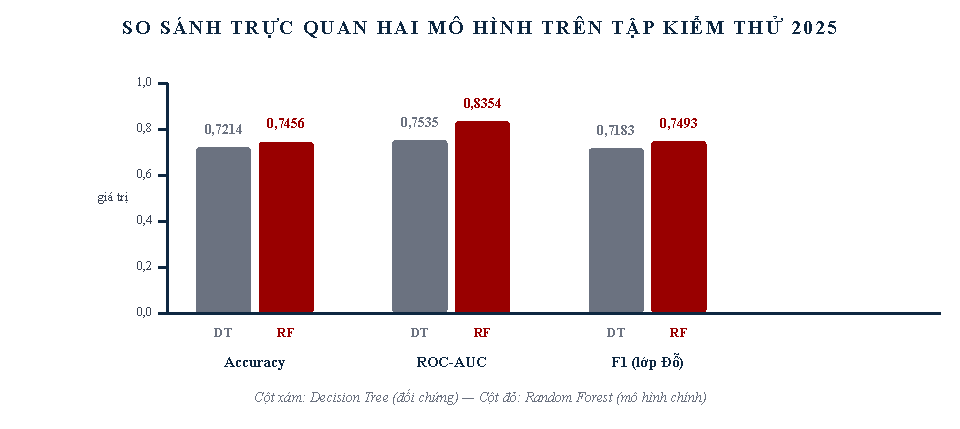
\includegraphics[width=0.92\textwidth]{figs/svg/h-model-bars.pdf}
\caption{So sánh trực quan bốn chỉ số của Decision Tree và Random Forest trên tập kiểm thử 2025.}
\label{fig:model-bars}
\end{figure}

Trong Hình~\ref{fig:model-bars}, cột xám là mô hình đối chứng và cột đỏ là mô hình
chính. Ba nhóm đầu (Accuracy, ROC-AUC, F1) đều là chỉ số ``càng cao càng tốt'' nên
cột đỏ đứng cao hơn là dấu hiệu tích cực. Riêng Brier là chỉ số ``càng thấp càng
tốt'', nên cột đỏ thấp hơn mới là kết quả mong muốn; khoảng cách ở nhóm này lớn hơn
hẳn ba nhóm còn lại, cho thấy lợi ích của Random Forest tập trung vào độ hiệu chuẩn
xác suất.

Bảng~\ref{tab:chi-tiet-lop} đi sâu vào từng lớp dự đoán, vì Accuracy tổng thể có thể
che khuất sự đánh đổi giữa hai loại lỗi.

\begin{table}[H]
\centering
\caption{Chi tiết Precision và Recall theo từng lớp của hai mô hình trên tập kiểm thử 2025.}
\label{tab:chi-tiet-lop}
\small
\begin{tabularx}{\textwidth}{@{}>{\raggedright\arraybackslash}p{3.5cm}
  >{\centering\arraybackslash}p{2.4cm}
  >{\centering\arraybackslash}p{2.4cm}
  >{\centering\arraybackslash}p{2.4cm}
  >{\centering\arraybackslash}p{2.4cm}@{}}
\toprule
\rowcolor{gray100}\bfseries\color{daunavy}Mô hình / Lớp &
\bfseries\color{daumaroon}Precision &
\bfseries\color{daumaroon}Recall &
\bfseries\color{daunavy}Precision &
\bfseries\color{daunavy}Recall \\
\midrule
 & \multicolumn{2}{c}{\bfseries\color{daumaroon}Lớp Đỗ} & \multicolumn{2}{c}{\bfseries\color{daunavy}Lớp Trượt} \\
\midrule
Decision Tree (đối chứng) & 0,8006 & 0,6514 & 0,6581 & 0,8053 \\
Random Forest (chính)     & \textbf{0,8098} & \textbf{0,6973} & \textbf{0,6887} & 0,8035 \\
\bottomrule
\end{tabularx}
\end{table}

Bảng~\ref{tab:chi-tiet-lop} giải thích vì sao Accuracy chỉ tăng 2,42 điểm phần trăm
trong khi ROC-AUC tăng tới 8,19 điểm. Với lớp Đỗ, Random Forest tăng đồng thời cả
Precision (0,8006 lên 0,8098) và Recall (0,6514 lên 0,6973), tức là vừa báo đúng hơn
vừa bỏ sót ít hơn. Với lớp Trượt, Precision tăng từ 0,6581 lên 0,6887 còn Recall gần
như giữ nguyên (0,8053 xuống 0,8035). Cách đánh đổi này phù hợp với mục đích sử dụng:
hệ thống cần hạn chế việc báo nhầm một nguyện vọng là ``an toàn'' khi thực tế rủi ro,
nên ưu tiên Precision của lớp Trượt, trong khi vẫn không đánh mất khả năng cảnh báo.

Ba điểm đọc quan trọng từ hai bảng trên:
\begin{itemize}[leftmargin=1.6em, itemsep=2pt]
  \item \textbf{ROC-AUC tăng 0,0819} (0,7535 $\rightarrow$ 0,8354): khả năng xếp hạng Đỗ/Trượt cải thiện rõ rệt nhờ trung bình 100 cây thay vì một cây đơn.
  \item \textbf{Brier giảm 0,0787} (0,2550 $\rightarrow$ 0,1763): xác suất dự đoán hiệu chuẩn tốt hơn, quan trọng vì hệ thống dùng giá trị $p$ trực tiếp để phân tầng.
  \item \textbf{Recall lớp Đỗ tăng 0,0459} trong khi Recall lớp Trượt giữ nguyên ($\approx$ 0,80): mô hình chính bắt được nhiều cơ hội đỗ hơn mà không đánh đổi khả năng cảnh báo trượt.
\end{itemize}

\subsection{Tầm quan trọng đặc trưng}

Bảng~\ref{tab:fi} trích 6 đặc trưng đóng góp lớn nhất từ \code{feature\_importances\_}
của Random Forest.

\begin{table}[H]
\centering
\caption{Mức đóng góp của 6 đặc trưng quan trọng nhất.}
\label{tab:fi}
\resizebox{0.85\textwidth}{!}{%
\begin{tabular*}{\textwidth}{@{\extracolsep{\fill}}>{\bfseries\color{daunavy}}l c l}
\toprule
\rowcolor{gray100}\bfseries\color{daunavy}Đặc trưng & \bfseries\color{daumaroon}Mức đóng góp & \bfseries\color{daunavy}Ý nghĩa \\
\midrule
\code{margin}        & 0,6060 & Khoảng cách điểm thi so với chuẩn mới nhất \\
\code{diem_thi}      & 0,2181 & Điểm năng lực tuyệt đối của thí sinh \\
\code{diem_moi_nhat} & 0,0509 & Mốc chuẩn cạnh tranh gần nhất \\
\code{diem_tb}       & 0,0425 & Mặt bằng chuẩn dài hạn \\
\code{bien_dong}     & 0,0164 & Biên độ rủi ro dao động \\
\code{xu_huong}      & 0,0164 & Độ dốc cạnh tranh qua hồi quy \\
\bottomrule
\end{tabular*}}
\end{table}

Bảng~\ref{tab:fi} được trích xuất trực tiếp từ thuộc tính \code{feature\_importances\_}
của mô hình sau khi huấn luyện, không phải đánh giá chủ quan của người viết. Giá trị
trong bảng là mức giảm độ bất thuần trung bình mà mỗi đặc trưng đóng góp trên toàn bộ
100 cây, chuẩn hóa để tổng bằng 1. Hai đặc trưng \code{margin} và \code{diem\_thi}
chiếm hơn 82\% tổng mức đóng góp, xác nhận trực giác tuyển sinh: khoảng cách tương đối
và năng lực tuyệt đối quyết định phần lớn kết quả. Nhóm đặc trưng lịch sử
(\code{diem\_moi\_nhat}, \code{diem\_tb}, \code{bien\_dong}, \code{xu\_huong}) đóng
vai trò hiệu chỉnh rủi ro, giúp phân biệt các ngành cùng mức \code{margin} nhưng độ ổn
định khác nhau.

Hình~\ref{fig:feature-importance} biểu diễn đầy đủ mười nhóm đặc trưng thay vì chỉ
sáu dòng trong bảng.

\begin{figure}[H]
\centering
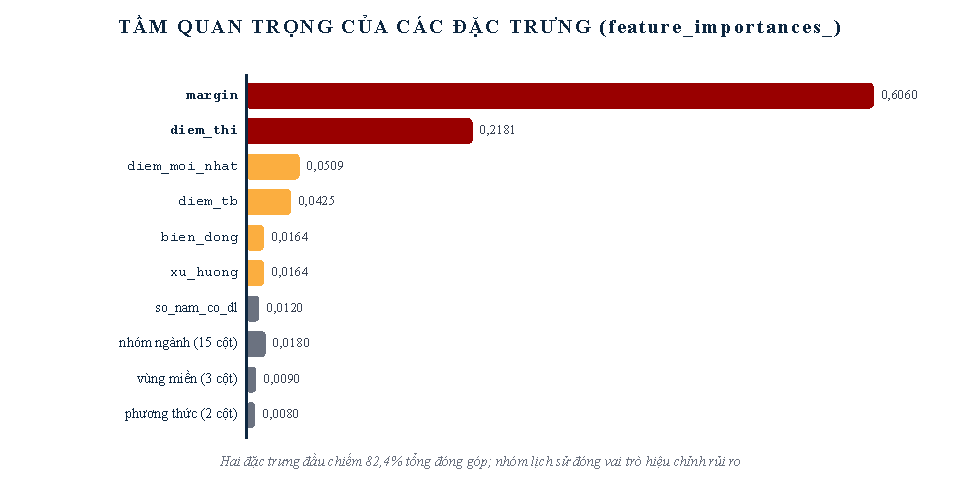
\includegraphics[width=0.92\textwidth]{figs/svg/h-feature-importance.pdf}
\caption{Mức đóng góp của toàn bộ các nhóm đặc trưng trong mô hình Random Forest.}
\label{fig:feature-importance}
\end{figure}

Hình~\ref{fig:feature-importance} cho thấy một điểm mà Bảng~\ref{tab:fi} không thể
hiện: 20 cột one-hot (15 nhóm ngành, 3 vùng miền, 2 phương thức) cộng lại chỉ chiếm
khoảng 3,5\% mức đóng góp, thấp hơn cả \code{diem\_tb}. Kết quả này không có nghĩa
các cột đó vô dụng --- chúng vẫn cần thiết để mô hình phân biệt ngành có cùng
\code{margin} --- mà cho thấy thông tin phân loại chủ yếu đóng vai trò điều chỉnh biên
chứ không quyết định xu hướng chính. Đây cũng là lý do vì sao việc tăng số chiều từ 10
lên 27 không làm mô hình kém đi: chi phí thêm 17 cột one-hot là rất nhỏ so với lượng
thông tin mà hai đặc trưng số trung tâm mang lại.

\section{So sánh với các công cụ tra cứu hiện có}

Để thấy rõ vị trí của Uni Connect, Bảng~\ref{tab:so-sanh-congcu} đối chiếu bảy nhóm
chức năng của hệ thống với ba nhóm công cụ mà thí sinh thường dùng: cổng thông tin
tuyển sinh của trường, các trang báo tổng hợp điểm chuẩn và các ứng dụng tư vấn có
thu phí. Việc so sánh chỉ dựa trên chức năng quan sát được, không dựa trên số liệu
người dùng của các bên.

\begin{table}[H]
\centering
\caption{Đối chiếu chức năng giữa Uni Connect và các nhóm công cụ tra cứu hiện có.}
\label{tab:so-sanh-congcu}
\small
\begin{tabularx}{\textwidth}{@{}>{\raggedright\arraybackslash}p{4.1cm}
  >{\centering\arraybackslash}p{1.9cm}
  >{\centering\arraybackslash}p{2.1cm}
  >{\centering\arraybackslash}p{1.9cm}
  >{\centering\arraybackslash}p{1.6cm}@{}}
\toprule
\rowcolor{gray100}\bfseries\color{daunavy}Chức năng &
\bfseries\color{daunavy}Cổng trường &
\bfseries\color{daunavy}Trang tổng hợp &
\bfseries\color{daunavy}Ứng dụng tư vấn &
\bfseries\color{daumaroon}Uni Connect \\
\midrule
Tra cứu điểm chuẩn nhiều năm & Một trường & Có & Có & Có \\
Gom dữ liệu toàn quốc một chỗ & Không & Một phần & Một phần & Có \\
Xác suất trúng tuyển theo hồ sơ & Không & Không & Có & Có \\
Phân tầng An toàn / Vừa sức / Thử sức & Không & Không & Một phần & Có \\
Lời giải thích kèm từng gợi ý & Không & Không & Không & Có \\
Lưu hồ sơ và lịch sử gợi ý & Không & Không & Có & Có \\
Cập nhật dữ liệu năm mới, huấn luyện lại & Không & Không & Không & Có \\
Mã nguồn mở, tự vận hành & Không & Không & Không & Có \\
\bottomrule
\end{tabularx}
\end{table}

Bảng~\ref{tab:so-sanh-congcu} cho thấy không nhóm công cụ nào có đủ cả bốn đặc điểm
mà đồ án hướng tới: dữ liệu gom một chỗ, xác suất tính theo hồ sơ cá nhân, phân tầng
kèm lời giải thích và khả năng tự cập nhật dữ liệu. Cổng thông tin của từng trường có
dữ liệu chính xác nhất nhưng chỉ phục vụ một trường và không có công cụ định lượng
rủi ro. Các trang tổng hợp giải quyết được bài toán tra cứu nhưng dừng ở việc hiển thị
bảng điểm thô. Ứng dụng tư vấn có thu phí tiến gần hơn ở khâu tính xác suất, nhưng
phần giải thích thường là câu văn cố định và người dùng không kiểm chứng được căn cứ.
Khoảng trống đó chính là lý do đồ án chọn hướng tiếp cận minh bạch: mọi con số dẫn
đến quyết định phân tầng đều hiển thị lại cho người dùng.

\section{Bàn luận}

Khoảng cách 2,42 điểm phần trăm Accuracy giữa hai mô hình nhỏ hơn khoảng cách ROC-AUC
(8,19 điểm), cho thấy lợi ích lớn nhất của Random Forest nằm ở chất lượng xếp hạng và
hiệu chuẩn xác suất chứ không chỉ nhãn cứng. Đây đúng là khía cạnh hệ thống cần nhất
vì quyết định phân tầng phụ thuộc toàn bộ vào thứ tự và giá trị $p$.

Phân tích ca sai cho thấy lỗi tập trung tại vùng \code{margin} gần 0 (từ $-0{,}5$ đến
$+0{,}5$): thí sinh ngang điểm chuẩn, nơi nhiễu tuyển sinh năm đơn lẻ (chỉ tiêu, phổ
điểm) át tín hiệu lịch sử. Đây là vùng hệ thống cố tình đẩy vào tầng Vừa sức kèm cảnh
báo biến động, thay vì khẳng định chắc chắn.

\section{Hạn chế}

\begin{itemize}[leftmargin=1.6em, itemsep=2pt]
  \item \textbf{Nhãn giả lập, không phải đỗ/trượt thật:} 11 mức \code{DELTAS} đối xứng chỉ xấp xỉ phân phối thí sinh; nhóm điểm xa chuẩn ($\pm 3{,}0$) dễ phân loại làm phồng Accuracy tổng thể.
  \item \textbf{Giới hạn hai phương thức:} Chưa xử lý đánh giá năng lực, đánh giá tư duy, chứng chỉ ngoại ngữ do khác thang điểm.
  \item \textbf{Nhiễu năm đơn lẻ:} Ngành mới mở, ngành đổi chỉ tiêu đột biến hoặc năm thiếu dữ liệu khiến \code{xu\_huong} và \code{bien\_dong} kém ổn định; hệ thống hiện gắn cờ ``dữ liệu mỏng'' thay vì dự báo mù.
  \item \textbf{Chưa kiểm thử tải đồng thời:} Đo 0,42 giây thực hiện trên truy vấn đơn; chưa đo tải hàng trăm người dùng song song mùa cao điểm.
\end{itemize}

\section{Tổng kết chương}

Chương này đã trình bày phần hiện thực và đo lường của đồ án: môi trường triển khai
với cấu hình tối thiểu 1 vCPU và 2~GB RAM, sáu bước của pipeline dữ liệu ngoại tuyến,
ba cấp độ kiểm thử với sáu ca chức năng đều đạt, và kết quả thực nghiệm của mô hình
trên tập kiểm thử độc lập năm 2025. Random Forest đạt Accuracy 74,56\%, ROC-AUC
0,8354 và Brier 0,1763, vượt mô hình đối chứng ở cả bốn chỉ số. Những hạn chế còn lại
--- chủ yếu là nhãn giả lập và phạm vi hai phương thức xét tuyển --- được tổng hợp ở
cuối chương và là cơ sở cho các hướng phát triển trình bày ở
Chương~\ref{ch:ketluan}.
